\documentclass[pdftex,11pt,a4paper]{article} % or extarticle

% *** PERSONAL & PAPER INFO ***
\newcommand{\sAuthors}{Artem Chirkin, Lukas Treyer, Michael Franzen}
\newcommand{\sTitle}{LC2 Specification}
\newcommand{\sSubject}{\sTitle}
\newcommand{\sKeywords}{Luci, middleware, json, geojson, planning}

% *** ACRONYMS ***
\usepackage{acronym}
%\acrodef{label}[acronym]{written out form}
\acrodef{Luci}{Lightweight Urban Computation Interchange}

% ----------------------------------------------------------------------------
% *** METADATA & TITLE ***
\usepackage[pdfauthor={\sAuthors},
            pdftitle={\sTitle},
            pdfsubject={\sSubject},
            pdfkeywords={\sKeywords},
            pdfproducer={Latex with hyperref},
            pdfcreator={pdflatex}]{hyperref}
\author{\sAuthors}
\title{\sTitle}

% *** GRAPHICS RELATED PACKAGES ***
\usepackage[pdftex]{graphicx}
\usepackage{epstopdf}
\usepackage{wrapfig}
\usepackage{subcaption}
\usepackage{bytefield}
\usepackage{msc}
\graphicspath{{resources/}}

% *** MATH PACKAGES ***
\usepackage{amsfonts}
\usepackage[cmex10]{amsmath}
% *** PDF, URL AND HYPERLINK PACKAGES ***
\usepackage{url}

% *** PAGE DIMENSIONS ***
\usepackage{geometry}
\geometry{top=1.0in, bottom=1.0in, left=1.0in, right=1.0in}
%\usepackage[section]{placeins} % force images to be within sections
\usepackage{parskip} % nicer indents in paragraphs
\usepackage{indentfirst} % add indent at first paragraph of the section
\usepackage{paralist} % denser lists

% making possible to execute arbitrary comands within the document
% \usepackage{bashful}
% \begingroup\makeatletter\endlinechar=\m@ne\everyeof{\noexpand}
% \edef\x{\endgroup\def\noexpand\TeXpath{\@@input|"ls ~/Documents" }}\x

% *** COMMENTING ***
%\usepackage[table]{xcolor}
\newcommand{\comment}[1]{{\color{red} #1 }}

% *** JAVASCRIPT LISTINGS ***

\usepackage{listings}
\definecolor{lightgray}{rgb}{.98,.98,.98}
\definecolor{darkgray}{rgb}{.4,.4,.4}
\definecolor{purple}{rgb}{0.65, 0.12, 0.82}

\lstdefinelanguage{JSON}{
  keywords={string,long,jsonGeometry,boolean,any,object,number,list,json,integer},
  keywordstyle=\color{blue}\bfseries,
  ndkeywords={OPT, XOR, MANY},
  ndkeywordstyle=\color{darkgray}\bfseries,
  identifierstyle=\color{black},
  sensitive=false,
  comment=[l]{//},
  morecomment=[s]{/*}{*/},
  commentstyle=\color{purple}\ttfamily,
  stringstyle=\color{red}\ttfamily,
  morestring=[b]',
  morestring=[b]"
}

\lstset{
   language=JSON,
   backgroundcolor=\color{lightgray},
   extendedchars=true,
   basicstyle=\footnotesize\ttfamily,
   showstringspaces=false,
   showspaces=false,
   numbers=left,
   numberstyle=\footnotesize\color{darkgray},
   numbersep=9pt,
   tabsize=2,
   breaklines=true,
   showtabs=false,
   captionpos=b
}

\usepackage{enumitem}
\setlistdepth{9}

\setlist[itemize,1]{label=$\bullet$}
\setlist[itemize,2]{label=$\bullet$}
\setlist[itemize,3]{label=$\bullet$}
\setlist[itemize,4]{label=$\bullet$}
\setlist[itemize,5]{label=$\bullet$}
\setlist[itemize,6]{label=$\bullet$}
\setlist[itemize,7]{label=$\bullet$}
\setlist[itemize,8]{label=$\bullet$}
\setlist[itemize,9]{label=$\bullet$}

\renewlist{itemize}{itemize}{9}

% *** DOCUMENT STARTS ***
\begin{document}
\maketitle
\tableofcontents
\section*{Changelog}
\begin{itemize}
  \item 2016-08-05: First draft
\end{itemize}
\clearpage


% up here was the title, the document content starts here
% ----------------------------------------------------------------------------

\section{Introduction}

\subsection{Notes}
The words "MUST", "MUST NOT", "REQUIRED", "SHALL", "SHALL NOT", "SHOULD", "SHOULD NOT", "RECOMMENDED", "MAY", and "OPTIONAL" are used in accordance to \href{https://www.ietf.org/rfc/rfc2119.txt}{RFC2119}.

\subsection{Understanding the document}

\subsection{Editing the document}
\label{sec:editing}

The document contains a number of JSON or GeoJSON listings representing content of \ac{Luci} actions.
In the listings we use the following coloring scheme:
%
\begin{itemize}
\item Key names are shown in black (e.g. \texttt{action});
\item Reserved keywords, such as value types are shown in blue (e.g. \texttt{\color{blue}string});
\item Fixed strings constants are shown in red (e.g. \texttt{\color{red}"create\_scenario"});
\item Additional structural keywords are shown in grey
(e.g. \texttt{\color{darkgray}OPT} means the key-value pair is optional, \texttt{\color{darkgray}XOR} before several key-value pairs means exactly one alternative).
\item Comments are in purple, separated by double slash (e.g. \texttt{\color{purple}// comment})
\end{itemize}
%
If there is a missing reserved keyword, you can add it into tex file annotation (\texttt{keywords} or \texttt{ndkeywords} lists in \texttt{lstdefinelanguage} command).

\clearpage

\section{Service API}
\label{ch:serviceapi}

Luci is primarily intended to connect machines in a LAN. Luci works as a TCP server, and all remote services and clients are TCP clients. In the beginning, a service registers itself in Luci, and then Luci sends run requests to the service from time to time. The service on the other hand keeps Luci updated of its current status.

\subsection{Registering a Service}

For registering a service in Luci, a set of three parameters \textbf{must} be implemented into the service and connect to Luci using the built-in service \texttt{RemoteRegister} (Appendix \ref{ch:builtinservices:RemoteRegister}).

The three required fields are
\begin{itemize}
  \item \texttt{serviceName}: The service name as a string
  \item \texttt{description}: The service description as a string
  \item \texttt{exampleCall}: An example call to the service as json encoded string
\end{itemize}

If a service accepts input arguments or outputs data, two additional parameters \textbf{can} be provided:
\begin{itemize}
  \item \texttt{input}: A json-schema that specifies the service input.
  \item \texttt{output}: A json-schema that specifies the service output
\end{itemize}

\subsubsection{JSON-Schema}

The schema for service inputs and outputs is a dictionary assigning each argument its type. A basic example schema is given in listing \ref{lst:schema}. A json-dictionary is valid for this schema if it contains the keys \texttt{foo}, \texttt{bar} and \texttt{baz} and assigns a number, string and boolean to them, respectively.
\begin{lstlisting}[caption={JSON Schema}, label={lst:schema}]
  {
    foo : number,
    bar : string,
    baz : boolean
  }
\end{lstlisting}

Arguments can be made optional and mutually exclusive using the prefixes OPT and XOR. In listing \ref{lst:schemaadvanced-optional}, only the field \texttt{foo} is obligatory. A valid JSON dictionary \textbf{must} contain the key \texttt{foo} and \textbf{can} contain the key \texttt{bar}.
\begin{lstlisting}[caption={JSON Schema with optional arguments}, label={lst:schemaadvanced-optional}]
  {
    foo : number,
    OPT bar : string
  }
\end{lstlisting}

Finally, consecutive arguments can be mutually exclusive. In listing \ref{lst:schemaadvanced-xor} the arguments \texttt{baz1}, \texttt{baz2}, \texttt{baz3} are mutually exclusive, indicating that exactly one of the three must be included.
\begin{lstlisting}[caption={JSON Schema with mutually exclusive arguments}, label={lst:schemaadvanced-xor}]
{
  XOR baz1 : boolean,
  XOR baz2 : boolean,
  XOR baz3 : boolean
}
\end{lstlisting}

\subsubsection{Example Register-message}
Listing \ref{lst:register-service} shows an example message how to register a service named \emph{ExampleService}. The schema in the section \texttt{inputs} indicates, that the service takes up to 2 input values: an obligatory number in the field \texttt{obligatory\_input} and
a string in the field \texttt{optional\_input}. The OPT-keyword indicates that the latter field is not a required one for the service to run.

After its execution, the service then outputs a dictionary containing the following keys:
\begin{itemize}
  \item \texttt{obligatory\_output} which is assigned a string value
  \item \texttt{output\_value1} \textbf{or} \texttt{output\_value2}. Only one of the keys is allowed to be included in the outputs.
  \item \texttt{optional\_output} which is a boolean and \textbf{optional}. In some cases, the service might output this value and in other cases it might omit it.
\end{itemize}

\begin{lstlisting}[caption={Registering a service}, label={lst:register-service}]
{
  run : "RemoteRegister",
  description : "I am an exemplary service",
  serviceName : "ExampleService",
  callID : 1,
  inputs : {
    obligatory_input : number,
    OPT optional_input : string
  },
  outputs : {
    obligatory_output : string,
    XOR output_value1 : number,
    XOR output_value2 : number.
    OPT optional_output : boolean
  },
  exampleCall : {
    {
      run : "ExampleService",
      optional_input : "foo",
      obligatory_input : 12
    }
  }
}
\end{lstlisting}

The whole message is sent as a \emph{run}-message (see section \ref{sec:runandcancel}) to the pseudo-service \emph{RemoteRegister}. Afterwards, Luci is aware of the service and associates the service \emph{ExampleService} with the IP from which this registration message originated.

\subsection{Run and Cancel}\label{sec:runandcancel}
When a client sends a message in the form
\begin{lstlisting}
{
  run: string, // the service name.
  callID: integer // a unique random number identifying the session
}
\end{lstlisting}
to Luci, Luci simply forwards this message to the service. The service \textbf{MAY} returns with a message containing in its run id:
\begin{lstlisting}
{
  newCallID: number, // the newly generated callID
  callID: integer // the same callID, it has priority over newCallID
}
\end{lstlisting}
If a client requests to stop the execution of a certain service call, he sends the following message which is subsequently forwarded to and handled by the service.
\begin{lstlisting}
{
  cancel: number, // the callID
  callID: integer // the same callID, it has priority over newCallID
}
\end{lstlisting}


\subsection{Result, Error and Progress}
Without any notification of Luci, the service is responsible of keeping Luci updated of the service's current status. The result is returned when the service is finished and is formatted in the following way:

\begin{lstlisting}
{
  result: json, // the result as specified in the output field upon service registration
  callID: integer
}
\end{lstlisting}

From time to time, the service might want to keep Luci updated of it's progress. If the progress equals 0, the service has been ordered to start.
\begin{lstlisting}
{
  progress: integer,
  callID: integer,
  OPT intermediateResult: json // some result, it is optional.
}
\end{lstlisting}

Finally, if an error occured, the service will provide an error message to Luci:
\begin{lstlisting}
{
  error: string,
  callID: integer
}
\end{lstlisting}

\subsection{Attachments}

Luci messages can contain binary data. It is attached to messages as byte arrays. Every message must contain a JSON "header", attachments are optional. The UTF8 encoded JSON header is human-readable; a complete luci message consists of a json string and a thin binary wrapper around the json header plus a binary attachements part.

Usually binary attachments should be referenced in a header using a special attachment description. Here is a convention for JSON format of such description:

\begin{lstlisting}
{
  format: string, // e.g. "binary" or "4-byte float array"
  attachment: {
    length: number, // length of attachments in bytes
    checksum: string, // MD5 checksum
    position: integer // starting at 1; 0 = undefined position
  }
  OPT name: string,
  ANY key: string
}
\end{lstlisting}

Attachments can be referenced multiple times in a JSON header. Attachments - if they need to be forwarded to only one service - are forwarded directly to remote services, i.e. Luci will not wait until the whole attachment is being transferred to Luci before sending it to a remote service.

\subsection{Geometry}
Similar to attachments a JSON header can also contain JSON encoded geometry like GeoJSON. Since there are several JSON based geometry formats (e.g. TopoJSON) a JSONGeometry object must follow this structure:

\begin{lstlisting}
{
  format: string, // e.g. "binary" or "4-byte float array"
  geometry: json, // format specific
  OPT name: string,
  OPT crs: string, // reference system
  OPT attributeMap: json,
}
\end{lstlisting}

\section{Low-Level Networking}
\label{ch:networking}

\begin{figure}[h!]
  \centering
  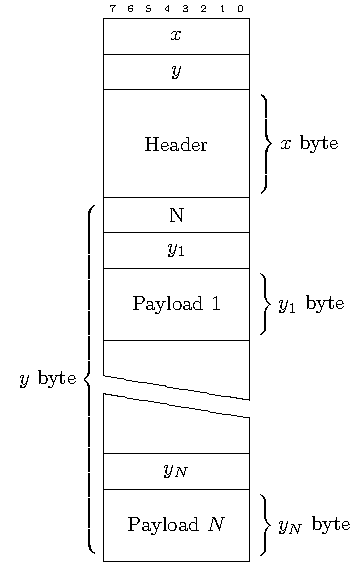
\includegraphics{bin/assets/binary-message-format.pdf}
  \caption{LC2 Message}
  \label{fig:lc2binary}
\end{figure}

\clearpage

\section{Scenario Services}
\label{ch:scenarios}

\ac{Luci} uses GeoJSON format to represent scenario geometry.
The format declares geometry information syntax, but does not declare consistent naming and geometry type mappings for \ac{Luci} scenario entities, such as buildings, roads, etc.
This document aims at providing guidelines on usage of \ac{Luci} scenarios in \ac{Luci} clients and services.

\paragraph{A note on jsonGeometry data type}
The word \texttt{geometry} in \ac{Luci} specification has two different meanings.
On the one hand it is a name of the key that occurs from time to time in \ac{Luci} actions.
On the other hand it is a name of a pre-defined data type that represents scenario geometry in JSON format.
To resolve this ambiguity, in current document we use word \texttt{geometry} to represent the name of the key, and \texttt{\color{blue}jsonGeometry} to represent the data type.
This differentiation does not introduce any changes to the existing JSON messages.

\subsection{\acs{Luci} scenario actions}
\label{ch:scenarios:actions}

% {"name":"shp_file_test","action":"create_scenario","geometry":{"anl.dbf":{"format":"dbf","attributeMap":{"geomid":"objectid","timestampformat":"YYYY","timestamp":"yearofchan"},"streaminfo":{"checksum":"48AC6C5CD751A525778A144EB66727","length":3138,"order":2}},"anl.shp":{"format":"shp","streaminfo":{"checksum":"39FBD5108DED0FF5637721A4820C484","length":1444,"order":1}},"anl.shx":{"format":"shx","streaminfo":{"checksum":"6B6F93D87FB73FF1AB92C3BD2938D2C","length":484,"order":3}}}}

To send geometry to \ac{Luci}, we wrap it in the structure that is shown in listing~\ref{json:geometry}
Special type \texttt{\color{blue}jsonGeometry} wraps various types of geometry processed by \ac{Luci}.
It allows to enclose arbitrary number of custom-named geometries (keys \texttt{KEY\_NAME\_N}) inline (GeoJSON) or in separate files (as binary attachments).
%
\begin{lstlisting}[caption={structure of \texttt{\color{blue}jsonGeometry} data type}, label={json:geometry}]
{
	/* key name is an arbitrary string.
	   The convention is to name it by filename of a file,
	   or arbitraryname.geojson in case of GeoJSON geometry */
	KEY_NAME_1 :
		XOR { // "in-line" geometry
			format   : string // "GeoJSON", later add also TopoJSON, CurveJSON, ...
			geometry : object // GeoJSON FeatureCollection
			OPT crs  : string // name of a crs
			OPT attributeMap : { // mapping between Luci and foreign types
				LUCI_ATTRIBUTE_NAME : FOREIGN_ATTRIBUTE_NAME,
				...
			}
		}
		XOR { // "streaminfo" - attachment description
			format     : string // shp | shx | dbf | any other file format?
			streaminfo : {
				checksum : string // MD5 sum of an attached binary data
				length : long // length of the attached binary data
				order : long // number of attachment (starts with 1)
			}
			OPT crs    : string // name of a crs
			OPT attributeMap : { // mapping between Luci and foreign types
				LUCI_ATTRIBUTE_NAME : FOREIGN_ATTRIBUTE_NAME,
				...
			}
		},
	KEY_NAME_2 : ...,
	...
}
\end{lstlisting}
%
The type of object \texttt{geometry} is GeoJSON \texttt{FeatureCollection} -- the format that is described in GeoJSON specification\footnote{\url{http://geojson.org/geojson-spec.html}}.


%Note, according to \ac{Luci} specification, object \texttt{geometry} is exchangeable (\texttt{XOR}) with \texttt{streaminfo}; however, no examples of \texttt{streaminfo} are provided, so \texttt{streaminfo} is excluded from this document.
%Also file \path{spec/luci_spec_todo.pdf} shows the format a bit more clear (geojson vs streaminfo), but I am not sure which version is implemented right now in Luci.
%\comment{This is a question to Lukas. }

According to \path{spec/LuciSpecification.pdf},
\ac{Luci} provides three operations to work with scenarios:
\texttt{create\_scenario}, \texttt{update\_scenario}, and \texttt{get\_scenario}.
This document covers only GeoJSON geometry manipulation;
in this format individual entities are represented as \texttt{Feature} objects in \texttt{FeatureCollection}.
Each \texttt{Feature} has a property \texttt{geomID:\color{blue}long} that is given either by a client, or by \ac{Luci} (in case if client application does not specify property \texttt{geomID}).


Creating a scenario is done
via \texttt{create\_scenario} action shown in listing~\ref{action:createScenario}.
The action allows to specify a location (\texttt{projection}) and a geometry to put inside the new scenario.
\begin{lstlisting}[caption={JSON action structure for creating a scenario in \ac{Luci}}, label={action:createScenario}]
{
	action           : "create_scenario", // constant, represents the action
	name             : string, // name of the scenario
	OPT projection   : {
		XOR crs    : string, // name of a crs
		XOR bbox   : [ [number, number]   // top-left coords [lat, long]
		             , [number, number]], // bottom-right coords [lat, long]
	},
	OPT geometry     : jsonGeometry, // wrapper around various geometry types
	OPT switchLatLon : boolean // switch lat-long to long-lat in geometry
}
\end{lstlisting}


Listing~\ref{action:updateScenario} shows the action to update scenario geometry.
The action allows to change the name and the bounding box, as well as the geometry inside.
\begin{lstlisting}[caption={JSON action structure for updating a scenario in \ac{Luci}}, label={action:updateScenario}]
{
	action       : "update_scenario", // constant, represents the action
	ScID         : long, // ID of the scenario in Luci
	OPT name     : string, // set a new name for the scenario
	OPT bbox     : [ [number, number]   // top-left coords [lat, long]
	               , [number, number]], // bottom-right coords [lat, long]
	OPT geometry : jsonGeometry // wrapper around various geometry types
	OPT switchLatLon : boolean // switch lat-long to long-lat in geometry
}
\end{lstlisting}
\begin{itemize}
\item In order to add an entity to the scenario, one adds \texttt{Feature} into \texttt{FeatureCollection} (\texttt{geometry} object).
\item In order to modify an existing entity, one must specify its property \texttt{geomID} (if given \texttt{geomID} does not exist, the entity is added to the scenario, otherwise it is edited).
\item In order to delete a number of entities from the scenario, one adds an empty \texttt{Feature} into \texttt{FeatureCollection} that has a property \texttt{deleted\_geomIDs:[\color{blue}long\color{black}]} -- array of \texttt{geomID} for deletion.
\end{itemize}

Listing~\ref{action:getScenario} shows the action to get scenario geometry.
The action allows to specify the format of the data to (\ac{Luci} does transformation),
and get the geometry from the scenario at given time.
\begin{lstlisting}[caption={JSON action structure for getting a scenario from \ac{Luci}}, label={action:getScenario}]
{
	action             : "get_scenario", // constant, represents the action
	XOR scenarioname   : string // name of the scenario in Luci
	XOR ScID           : long, // ID of the scenario in Luci
	OPT format_request : string, // maybe we will change this later to "format"
	OPT crs            : string,
	OPT geomIDs        : [long], // select a subset of scenario objects
	OPT timerange      : { // time is a number - timestamp in unix format
		XOR until   : long,
		XOR from    : long,
		XOR between : [long,long],
		XOR exactly : long,
		OPT all     : boolean // include all versions (not only the last)
	}
}
\end{lstlisting}

\subsection{Scenario GeoJSON geometry}
\label{sec:services:scenario}

Although GeoJSON specification provides all necessary geometry primitives,
we need a more structured convention to define one-to-one mapping between the geometry and scenario entities.
\ac{Luci} does not generate an error for an input that does not follow it -- the convention only describes what kind of data structures services and clients should expect.

Section~\ref{ch:scenarios:standardrules} describes the rules assumed by \ac{Luci} when communicating with all services and clients.
Section~\ref{ch:scenarios:conventionalrules} describes the rules assumed by most applications, but not checked in \ac{Luci}.
Section~\ref{ch:scenarios:applicationrules} describes the application-specific rules.
Any service or client provider (\ac{Luci} user) may introduce a rule that is used in their application.
The providers are encouraged to add these rules into section~\ref{ch:scenarios:applicationrules}.
By an agreement in our team some of the rules go up from section~\ref{ch:scenarios:applicationrules} to section~\ref{ch:scenarios:conventionalrules}.
In case of wide usage they might be enforced in \ac{Luci}, thus moving one step up to section~\ref{ch:scenarios:standardrules}.

\subsubsection{Standardized Rules}
\label{ch:scenarios:standardrules}
Object \texttt{geometry} in listing~\ref{json:geometry} is assumed to be of type \texttt{FeatureCollection}.
Every entity is represented as a \texttt{Feature} inside that collection, and has a property \texttt{geomID:\color{blue}long} that is given by a client or \ac{Luci} (if the client omits the property).

\subsubsection{Conventional Rules}
\label{ch:scenarios:conventionalrules}

Some services require 3D objects, others use only 2D footprints.
To distinguish these two types of geometry, we agreed on using \texttt{Feature} property \texttt{layer}.
\begin{itemize}
\item Object (e.g. Building) -- a 3D geometry, represented as \texttt{Feature} with \texttt{geometry} field of type \texttt{Polygon} or \texttt{MultiPolygon}.
To be processed correctly by \ac{Luci} services, the object requires property \texttt{layer:\color{red}"buildings"}.
%
\item Footprint -- a 2D geometry, represented as \texttt{Feature} with \texttt{geometry}
field of type \texttt{Polygon} or \texttt{MultiPolygon}.
To be processed correctly by \ac{Luci} services, the footprint requires property \texttt{layer:\color{red}"footprints"}.
\end{itemize}


\subsubsection{Per-application Rules}
\label{ch:scenarios:applicationrules}

\paragraph{Web geometry modeler}
The application distinguishes dynamic and static geometry:
dynamic geometry can be edited, static geometry is only used for evaluation and visualization.
Thus, I propose an optional property \texttt{static:\color{blue}boolean}.
Absence of a property implies \texttt{static:\color{brown}false}.

\clearpage

\section{QUA-Compliance}
\label{ch:quacompliance}

To make a service compliant for use in the qua-kit, a service is subject to additional constraints that are described here.
A qua-view-compliant service must support one or more of following working modes:
\begin{itemize}
\item 
    \texttt{scenario} -- a service gets a scenario as input and returns a single result for a whole scenario;
\item 
    \texttt{objects} -- a service gets a scenario and ids of individual objects and returns a result per every object;
\item 
    \texttt{points} -- a service gets a scenario and a grid of points, and returns a result per each point on the grid;
\item 
    \texttt{new} -- a service updates or creates a new geometry.
\end{itemize}

\subsection{QUA-View-Compliance}

Defining a service being
\texttt{qua-view-compliant} means promising to follow a strict predefined format of service input, output, and parameters.
To declare a service \texttt{qua-view-compliant}, one needs to add \texttt{qua-view-compliant:true} flag in the root
of \texttt{RemoteRegister} JSON message sent to luci/helen at the start of a service execution.
To test if a service follows strictly the specification is a responsibility of a service developer.

\subsubsection{Optional parameters}

A \texttt{qua-view-compliant} service may have arbitrary number of optional parameters.
All optional parameters must be defined in an \texttt{inputs} object of \texttt{RemoteRegister} JSON message
using \texttt{paramName:paramType} syntax.
Valid parameter types are:
\begin{enumerate}
\item \texttt{boolean} -- either \texttt{true} or \texttt{false};
\item \texttt{number} -- any number type;
\item \texttt{string} -- a fixed string, must have a corresponding field in \texttt{constraints} object.
\end{enumerate}

\subsubsection{Constraints}

Parameters may have constraints defined on them.
These constraints are used by qua-view control panel to configure user input fields.
To define a constraint, one needs to use \texttt{constraints} object in the root of \texttt{RemoteRegister} JSON message
(see listing~\ref{lst:quaconstraints}).
\begin{lstlisting}[caption={qua-compliance -- parameter constraints}, label={lst:quaconstraints}]
{
  run : "RemoteRegister",
  ...
  qua-view-compliant : true,
  inputs : {
    ...
    mode : "string",
    constrainedInput1 : "number",
    constrainedInput2 : "string"
  },
  outputs : {
    ...
  },
  constraints : {
      mode: ["points", "scenario"],
      constrainedInput1 : {
          min : 42,
          integer : true
      },
      constrainedInput2 : ["hello", "world", "3rd option"]
  },
  ...
}
\end{lstlisting}

\paragraph{Number}
To describe constraints on a number type, one needs to create a JSON object with following (all optional) records:
\begin{itemize}
\item \texttt{min:number} -- minimum allowed value;
\item \texttt{max:number} -- maximum allowed value;
\item \texttt{def:number} -- default value visible in a viewer;
   \texttt{\begin{itemize}
   \item (min = undef, max = undef, def = undef): def = 0;
   \item (min = exist, max = undef, def = undef): def = min;
   \item (min = undef, max = exist, def = undef): def = max;
   \item (min = exist, max = exist, def = undef): def = (max - min) / 2;
   \end{itemize}}
\item \texttt{integer:boolean} -- whether to treat a number as an integer; default \texttt{integer:false}.
\end{itemize}

\paragraph{String}
To describe contraints on a string, one needs to create a JSON array of strings -- an enumeration of possible value.
Without a constraint object, a parameter accepts any string value;
with a constraint object, a parameter is displayed as a drop-down list of possible options
(see listing~\ref{lst:quaconstraints} constraints on a \texttt{constrainedInput2} input key).
The first option in a list is the default one.


\paragraph{Boolean}
One possible constraint for a boolean is a default value in qua-view.
Use \texttt{\{def:true\}} or \texttt{\{def:false\}} constructs.


\subsection{Execution modes}

The execution modes define how a service is visualized in qua-view.
Each mode dictates obligatory input and output parameters.
A service may support more than one execution modes.
At runtime, an execution mode is defined by \texttt{inputs} record \texttt{mode:string}.
A qua-view-compliant service must define \texttt{inputs/mode} field in \texttt{RemoteRegister} JSON message
and a corresponding constraint (the same way as optional parameters).

\subsubsection{points}

In this mode, qua-view generate a grid of points in 3D and sends them to a service together with scenario reference.
A service sends back floating point values for each point.
Then, qua-view visualizes the values as a coloured heat map.
The grid of points is sent in a binary attachment in form \texttt{XYZXYZ...XYZ}, 4 byte floating point value per coordinate
in Little Endian format (\texttt{float32}) -- $3 \cdot 4 n$ bytes in total, where $n$ is the number of points.
A service determines a number of points by the size of incoming data.
\begin{lstlisting}[caption={A qua-compliant service run request for mode \texttt{points}}, label={lst:quacompliantinput:points}]
{
  run : "RandomQUA",
  callID : 283,
  ScID : 123,
  mode : "points",
  points : {
    format : "float32 array",
    attachment {
      length : 3072,
      position : 1,
      checksum : "2929bead3ee3cf55113ec9aade2b6add"
    }
  }
}
\end{lstlisting}

\begin{lstlisting}[caption={A qua-compliant service output for mode \texttt{points}}, label={lst:quacompliantresult:points}]
{
  callID : 283,
  result : {
    units : "metre",
    values : {
      format : "float32 array",
      attachment : {
        length: 1024,
        checksum: "50752c7cb358a5fffd913d9aa3605433",
        position: 1
      }
    }
  }
}
\end{lstlisting}
A result of a service execution must contain following fields:
\begin{enumerate}
\item \texttt{units} -- any string, e.g. "metre", "kg", "mm/s", etc.;
\item \texttt{values} -- attachment object containing a reference to a blob of \texttt{float32} data;
 its size must be exactly $4 n$, where $n$ is the number of points received.
\end{enumerate}

\subsubsection{objects}

This mode is similar to \texttt{points} mode except instead of point coordinates a client (qua-view) sends ids of geometric objects
within a scenario.
Qua-view visualizes it by colouring objects according to the values received for each object.
A user also can click on a building and see exact numeric value received from a service.

A service in this mode has two obligatory inputs:
\begin{enumerate}
\item \texttt{ScID} -- id of a current scenario;
\item \texttt{objIds} -- an attachment reference to a binary blob of size $8n$, where $n$ is the number of objects to process by a service;
                         the blob consists of unsigned 8-byte integers in Little Endian format (\texttt{ulong64}) -- \texttt{geomID} of each object. 
\end{enumerate}
\begin{lstlisting}[caption={A qua-compliant service run request for mode \texttt{objects}}, label={lst:quacompliantinput:objects}]
{
  run : "RandomQUA",
  callID : 172,
  ScID : 123,
  mode : "objects",
  objIds : {
    format : "ulong64 array",
    attachment {
      length : 2048,
      position : 1,
      checksum : "50752c7cb358a5fffd913d9aa3605433"
    }
  }
}
\end{lstlisting}

A result of a service execution must contain following fields:
\begin{enumerate}
\item \texttt{units} -- any string, e.g. "metre", "kg", "mm/s", etc.;
\item \texttt{values} -- attachment object containing a reference to a blob of \texttt{float32} data;
 its size must be exactly $2 n$, where $n$ is the number of objects' \texttt{geomID} received.
\end{enumerate}
\begin{lstlisting}[caption={A qua-compliant service output for mode \texttt{objects}}, label={lst:quacompliantresult:objects}]
{
  callID : 172,
  result : {
    units : "metre",
    values : {
      format : "float32 array",
      attachment : {
        length: 1024,
        checksum: "2929bead3ee3cf55113ec9aade2b6add",
        position: 1
      }
    }
  }
}
\end{lstlisting}

\subsubsection{scenario}

A scenario execution mode returns only one value for a whole scenario.
The value can be an arbitrary string or a \texttt{.png} image (in attachment).
In either way, the result is displayed on a side panel in qua-view.

The only obligatory field in this mode is a scenario id \texttt{ScID}.
\begin{lstlisting}[caption={A qua-compliant service run request for mode \texttt{scenario}}, label={lst:quacompliantinput:scenario}]
{
  run : "RandomQUA",
  callID : 213,
  ScID : 125,
  mode : "scenario"
}
\end{lstlisting}

One possible result of a scenario-mode-service is a text string.
\begin{lstlisting}[caption={A qua-compliant service output for mode \texttt{scenario} (string output)}, label={lst:quacompliantresult:scenario}]
{
  callID : 213,
  result : {
    answer : "This scenario looks good! The goodness level is 9.125."
  }
}
\end{lstlisting}

Another possible result type is a \texttt{.png} image attached to a message.
Recommended size of an image is 512x512px.
An image may contain a graph or an arbitrary figure.
\begin{lstlisting}[caption={A qua-compliant service output for mode \texttt{scenario} (image output)}, label={lst:quacompliantresult:scenario}]
{
  callID : 213,
  result : {
    image : {
      format : "image/png",
      attachment : {
        length: 12623,
        checksum: "8329beex3ee3cf55113ec9aade2b6a02a",
        position: 1
      }
    }
  }
}
\end{lstlisting}


\subsubsection{new}

In this mode, a service updates or creates a new geometry.
It can be used by various geometry-generating services.
A \texttt{ScID} key is optional. This mode does not have obligatory parameters.
A service should write its output directly into scenario via luci/helen.
The output of a service must have following fields:
\begin{lstlisting}
result: {
  ScID : long, // the id of the newly created scenario
  timestamp_accessed : long, // optional - the timestamp at which the scenario was accessed if the ScID-field was set in the input
  timestamp_modified : long // the timestamp at which the new scenario was stored
}
\end{lstlisting}

\begin{lstlisting}[caption={A qua-compliant service run request for mode \texttt{new}}, label={lst:quacompliantinput:new}]
{
  run : "RandomQUA",
  callID : 244,
  mode : "new" // Note how the call does not contain a ScID
}
\end{lstlisting}

\begin{lstlisting}[caption={A qua-compliant service output for mode \texttt{new}}, label={lst:quacompliantresult:new}]
{
  callID : 244,
  result : {
    ScID : 1337,
    timestamp_accessed : 1472137755,
    timestamp_modified : 1472137758
  }
}
\end{lstlisting}

\subsection{Registering a service}

TODO: more explanations

\begin{lstlisting}[caption={Registering a QUA-compliant service}, label={lst:quacompliance}]
{
  run : "RemoteRegister",
  description : "I am a random service", // obligatory
  serviceName : "RandomQUA",
  callID : 1, // obligatory
  qua-view-compliant : true, // obligatory
  inputs : {
    OPT geomID : number, // obligatory for all modes except "new"
    mode : string, // obligatory
    points : attachment,
    some other input : number,
    some 4th input : number
  },
  outputs : {
    unit : string,
    mode : string,
    XOR value : number,
    XOR values : attachment,
    OPT scenario_id : long,
    OPT timestamp_accessed : int,
    OPT timestamp_modified : int
  }
  constraint : {
      some other input : {
          min : 42,
          max : 100,
          integer : true
      }
  },
  exampleCall : {
    {
      run : "RandomQUA",
      geomID : 123,
      mode : "points",
      points : {
        format : "float32 array",
        attachment {
          length : 100,
          position : 1,
          checksum : "2929bead3ee3cf55113ec9aade2b6add"
        }
      }
      some other input : 42,
      some 4th input : 13.37
    }
  }
}
\end{lstlisting}


\clearpage


\appendix

\section{Built-In Services}
\label{ch:builtinservices}

\subsection{AttachmentJSON}
\label{ch:builtinservices:AttachmentJSON}
Returns the json specification of attachments and json geometry objects.
\subsubsection*{Inputs:}
\begin{itemize}
  \small
    \item \textbf{run}: 
\begin{lstlisting}
AttachmentJSON
\end{lstlisting}
  \end{itemize}
\subsubsection*{Outputs:}
\begin{itemize}
  \small
    \item \textbf{XOR error}: 
\begin{lstlisting}
string
\end{lstlisting}
    \item \textbf{XOR progress}: 
\begin{lstlisting}
json
\end{lstlisting}
    \item \textbf{XOR result}: 
\begin{lstlisting}
{
  attachment: attachment, 
  jsongeometry: jsongeometry
}
\end{lstlisting}
  \end{itemize}

\subsection{Download}
\label{ch:builtinservices:Download}
Downloads
 a file from a given URL and stores is in Luci's attachment folder as 
\&lt;md5 checksum\&gt;.\&lt;format\&gt; 
\subsubsection*{Inputs:}
\begin{itemize}
  \small
    \item \textbf{run}: 
\begin{lstlisting}
Download
\end{lstlisting}
    \item \textbf{url}: the URL to be used
\begin{lstlisting}
string
\end{lstlisting}
  \end{itemize}
\subsubsection*{Outputs:}
\begin{itemize}
  \small
    \item \textbf{XOR error}: 
\begin{lstlisting}
string
\end{lstlisting}
    \item \textbf{XOR progress}: 
\begin{lstlisting}
json
\end{lstlisting}
    \item \textbf{XOR result}: 
\begin{lstlisting}
{
  checksum: string// the checksum in hexadecimal representation, 
  format: string// equals the string typically put as a file ending, 
  length: number// the length of the attachments as number of bytes
}
\end{lstlisting}
  \end{itemize}

\subsection{Exists}
\label{ch:builtinservices:Exists}
Tests whether a service with the given serviceName or a task with given taskID exists.
\subsubsection*{Inputs:}
\begin{itemize}
  \small
    \item \textbf{run}: 
\begin{lstlisting}
Exists
\end{lstlisting}
    \item \textbf{XOR instanceID}: 
\begin{lstlisting}
number
\end{lstlisting}
    \item \textbf{XOR serviceName}: the name of the service to be tested
\begin{lstlisting}
string
\end{lstlisting}
  \end{itemize}
\subsubsection*{Outputs:}
\begin{itemize}
  \small
    \item \textbf{XOR error}: 
\begin{lstlisting}
string
\end{lstlisting}
    \item \textbf{XOR progress}: 
\begin{lstlisting}
json
\end{lstlisting}
    \item \textbf{XOR result}: 
\begin{lstlisting}
{
  exists: boolean
}
\end{lstlisting}
  \end{itemize}

\subsection{FilterServices}
\label{ch:builtinservices:FilterServices}
Filters
 services according to a) its keys at a given recursion level, b) its 
types at a given recursion level or c) a given json template with values
 equal to 'null' meaning only keys are compared.
\subsubsection*{Inputs:}
\begin{itemize}
  \small
    \item \textbf{run}: 
\begin{lstlisting}
FilterServices
\end{lstlisting}
    \item \textbf{XOR jsonMatch}: 
\begin{lstlisting}
json
\end{lstlisting}
    \item \textbf{XOR keys}: 
\begin{lstlisting}
[
  string
]
\end{lstlisting}
    \item \textbf{XOR types}: 
\begin{lstlisting}
[
  string
]
\end{lstlisting}
    \item \textbf{OPT rcrLevel}: 
\begin{lstlisting}
number
\end{lstlisting}
  \end{itemize}
\subsubsection*{Outputs:}
\begin{itemize}
  \small
    \item \textbf{XOR error}: 
\begin{lstlisting}
string
\end{lstlisting}
    \item \textbf{XOR progress}: 
\begin{lstlisting}
json
\end{lstlisting}
    \item \textbf{XOR result}: 
\begin{lstlisting}
{
  serviceList: [
    string
  ]
}
\end{lstlisting}
  \end{itemize}

\subsection{GetStartupTime}
\label{ch:builtinservices:GetStartupTime}
Returns the startup of time of Luci.
\subsubsection*{Inputs:}
\begin{itemize}
  \small
    \item \textbf{run}: 
\begin{lstlisting}
GetStartupTime
\end{lstlisting}
  \end{itemize}
\subsubsection*{Outputs:}
\begin{itemize}
  \small
    \item \textbf{XOR error}: 
\begin{lstlisting}
string
\end{lstlisting}
    \item \textbf{XOR progress}: 
\begin{lstlisting}
json
\end{lstlisting}
    \item \textbf{XOR result}: 
\begin{lstlisting}
{
  startupTime: number// in milliseconds since 1.1.1970
}
\end{lstlisting}
  \end{itemize}

\subsection{RemoteDeregister}
\label{ch:builtinservices:RemoteDeregister}
Deregisters
 a client from a service registration. This will cancel any running 
service call, cancel all subscriptions of this client and, if the 
service to be deregistered is the last remaining of its kind, its 
serviceName will be removedfrom the list of available services.
\subsubsection*{Inputs:}
\begin{itemize}
  \small
    \item \textbf{run}: 
\begin{lstlisting}
RemoteDeregister
\end{lstlisting}
  \end{itemize}
\subsubsection*{Outputs:}
\begin{itemize}
  \small
    \item \textbf{XOR error}: 
\begin{lstlisting}
string
\end{lstlisting}
    \item \textbf{XOR result}: 
\begin{lstlisting}
{
  deregisteredName: string// Intended to inform listeners about the service name that was deregistered, 
  id: number// int, the id that was deregistered, 
  nodeIP: string// Intended to inform listeners about the IP of the machine that deregistered the service, 
  remainsAvailable: boolean// boolean to indicate whether other services with the samename remain  available (true) or whether the service is being deleted from the listof  available services (false)
}
\end{lstlisting}
  \end{itemize}

\subsection{RemoteRegister}
\label{ch:builtinservices:RemoteRegister}
Registers a client as a service.
\subsubsection*{Inputs:}
\begin{itemize}
  \small
    \item \textbf{run}: 
\begin{lstlisting}
RemoteRegister
\end{lstlisting}
    \item \textbf{description}: 
\begin{lstlisting}
string
\end{lstlisting}
    \item \textbf{exampleCall}: Mandatory json object that shows an example call. Since OPT/XOR/ANY  modifiers are only allowed in in \& output specifications and not in  calls, an example call shows very clearly how a call could look like.
\begin{lstlisting}
json
\end{lstlisting}
    \item \textbf{serviceName}: mandatory string that identifies the service
\begin{lstlisting}
string
\end{lstlisting}
    \item \textbf{OPT id}: Optional int to be used to identify a remote service. E.g. for  viewer services it might be important to be able to identify remote  service instances. If the id is taken already an error will be thrown /  registration aborted.
\begin{lstlisting}
number
\end{lstlisting}
    \item \textbf{OPT inputs}: Optional json object holding the input description to be included by 'ServiceInfo' / the API
\begin{lstlisting}
json
\end{lstlisting}
    \item \textbf{OPT outputs}: Optional json object holding the output description to be included by 'ServiceInfo' / the API
\begin{lstlisting}
json
\end{lstlisting}
  \end{itemize}
\subsubsection*{Outputs:}
\begin{itemize}
  \small
    \item \textbf{XOR error}: 
\begin{lstlisting}
string
\end{lstlisting}
    \item \textbf{XOR result}: 
\begin{lstlisting}
{
  id: number// The int given as input or an int generated by Luci, 
  nodeIP: string// The IP of the client that was registered as a service (intended to inform listeners), 
  registeredName: string// Intended to inform listeners about the service name that was registered
}
\end{lstlisting}
  \end{itemize}

\subsection{ServiceControl}
\label{ch:builtinservices:ServiceControl}
Used
 to remotely administrate installed services on a selected machine or on
 allmachines having a 'ServiceControl' remote service running.
\subsubsection*{Inputs:}
\begin{itemize}
  \small
    \item \textbf{run}: 
\begin{lstlisting}
ServiceControl
\end{lstlisting}
    \item \textbf{XOR info}: get filtered information about either selected machines (nodes) or  about selectedserviceNames on all machines or full information about all  machines in case this value is 'null'
\begin{lstlisting}
{
  \null\: error, 
  {XOR nodes: {
    OPT threadPool: boolean, 
    XOR nodes: [
      string
    ], 
    XOR serviceNames: [
      string
    ]
  }
}
\end{lstlisting}
    \item \textbf{XOR install}: install files on either selected machines (nodes) or on all machines (services)
\begin{lstlisting}
{
  XOR nodes: {
    ANY IP: [
      attachment
    ]
  }, 
  XOR services: [
    attachment
  ]
}
\end{lstlisting}
    \item \textbf{XOR remove}: remove services identified by their name (serviceName) either on selected machines (nodes) or on all machines (services)
\begin{lstlisting}
{
  XOR nodes: {
    ANY IP: [
      string
    ]
  }, 
  XOR services: [
    string
  ]
}
\end{lstlisting}
    \item \textbf{XOR start}: startup a given number of services either globally or on selected machines (nodes)
\begin{lstlisting}
{
  XOR nodes: {
    ANY IP: {
      ANY serviceName: {
        \number\,: error, 
        {ANY id: {
          ANY id: string
        }
      }
    }
  }, 
  XOR services: {
    ANY serviceName: number
  }
}
\end{lstlisting}
    \item \textbf{XOR stop}: stop a given amount of services either globally or on specified machines (nodes).
\begin{lstlisting}
{
  XOR nodes: {
    ANY IP: {
      ANY serviceName: number
    }
  }, 
  XOR services: {
    ANY serviceName: number
  }
}
\end{lstlisting}
  \end{itemize}
\subsubsection*{Outputs:}
\begin{itemize}
  \small
    \item \textbf{XOR error}: 
\begin{lstlisting}
string
\end{lstlisting}
    \item \textbf{XOR result}: 
\begin{lstlisting}
{
  OPT errors: list// 'TODO' in case at least one of the items to  install/remove/start/stop produced an error this list contains one error  string per item, 
  XOR info: {
    OPT quickPool: {
      avgWaitingTime: number, 
      maxPoolSize: number, 
      numCalls: number, 
      poolSize: number, 
      waitingInQueue: number
    }, 
    OPT slowPool: {
      avgWaitingTime: number, 
      maxPoolSize: number, 
      numCalls: number, 
      poolSize: number, 
      waitingInQueue: number
    }, 
    XOR nodes: {
      ANY ip: {
        OPT installedServices: {
          ANY serviceName: {
            exec: string// to be run in console, 
            numRequestedCPUCores: number// 0 = using all available cores
          }
        }, 
        OPT system: {
          CPU: {
            archNumBits: number// int; 32 or 64, 
            endian: string// 'big' or 'little', 
            numCores: number
          }, 
          name: string, 
          osname: string, 
          osversion: string
        }, 
        services: {
          busy: {
            ANY serviceName: number
          }, 
          idle: {
            ANY serviceName: number
          }, 
          running: {
            ANY serviceName: number
          }
        }
      }
    }, 
    XOR services: {
      ANY serviceName: {
        OPT available: number// not busy, 
        OPT nodes: list// list of IPv4, 
        OPT running: number, 
        avgDuration: number// in milliseconds, 
        numCalls: number// how many times this service has been called already
      }
    }, 
    remoteSummary: {
      busy: number, 
      idle: number
    }
  }, 
  XOR installed: {
    ANY IP: [
      string
    ]
  }, 
  XOR removed: {
    ANY IP: [
      string
    ]
  }, 
  XOR started: {
    ANY IP: {
      ANY serviceName: number
    }
  }, 
  XOR stopped: {
    ANY IP: {
      ANY serviceName: number
    }
  }
}
\end{lstlisting}
  \end{itemize}

\subsection{ServiceHistory}
\label{ch:builtinservices:ServiceHistory}
Returns
 the history of a requested service as in number of calls and 
availableworkers either since startup time or during the requested 
period
\subsubsection*{Inputs:}
\begin{itemize}
  \small
    \item \textbf{run}: 
\begin{lstlisting}
ServiceHistory
\end{lstlisting}
    \item \textbf{serviceName}: 
\begin{lstlisting}
string
\end{lstlisting}
    \item \textbf{OPT period}: in seconds
\begin{lstlisting}
number
\end{lstlisting}
  \end{itemize}
\subsubsection*{Outputs:}
\begin{itemize}
  \small
    \item \textbf{XOR error}: 
\begin{lstlisting}
string
\end{lstlisting}
    \item \textbf{XOR progress}: 
\begin{lstlisting}
json
\end{lstlisting}
    \item \textbf{XOR result}: 
\begin{lstlisting}
{
  calls: {
    { callID: {
      callID: number, 
      idleTime: number, 
      readingTime: number, 
      runningTime: number, 
      timestamp: number, 
      writingTime: number
    }
  }, 
  workers: {
    { allWorkers: {
      allWorkers: number, 
      idleWorkers: number, 
      timestamp: number
    }
  }
}
\end{lstlisting}
  \end{itemize}

\subsection{ServiceInfo}
\label{ch:builtinservices:ServiceInfo}
Returns
 all known information on selected services such as a short description 
like this one, in- and output description and an example call. 
\subsubsection*{Inputs:}
\begin{itemize}
  \small
    \item \textbf{run}: 
\begin{lstlisting}
ServiceInfo
\end{lstlisting}
    \item \textbf{OPT inclDescr}: indicates whether descriptions such as this one should be included in the result
\begin{lstlisting}
boolean
\end{lstlisting}
    \item \textbf{OPT serviceNames}: Optional list of selected service names for which information should  be returned. If no such list is given, the result will show the  structure of general json structures such as 'attachment',  'jsongeometry'
\begin{lstlisting}
list
\end{lstlisting}
  \end{itemize}
\subsubsection*{Outputs:}
\begin{itemize}
  \small
    \item \textbf{XOR error}: 
\begin{lstlisting}
string
\end{lstlisting}
    \item \textbf{XOR result}: 
\begin{lstlisting}
{
  ANY serviceName: {
    OPT numNodes: number, 
    example: json, 
    inputs: json, 
    outputs: json
  }
}
\end{lstlisting}
  \end{itemize}

\subsection{ServiceList}
\label{ch:builtinservices:ServiceList}
Get a list of all loaded and registered services as a list of service names.
\subsubsection*{Inputs:}
\begin{itemize}
  \small
    \item \textbf{run}: 
\begin{lstlisting}
ServiceList
\end{lstlisting}
  \end{itemize}
\subsubsection*{Outputs:}
\begin{itemize}
  \small
    \item \textbf{XOR error}: 
\begin{lstlisting}
string
\end{lstlisting}
    \item \textbf{XOR progress}: 
\begin{lstlisting}
json
\end{lstlisting}
    \item \textbf{XOR result}: 
\begin{lstlisting}
{
  installed: list, 
  serviceNames: list
}
\end{lstlisting}
  \end{itemize}

\subsection{task.Create}
\label{ch:builtinservices:task.Create}
Create a task. A task corresponds to a node in the workflow diagram.
\subsubsection*{Inputs:}
\begin{itemize}
  \small
    \item \textbf{run}: 
\begin{lstlisting}
task.Create
\end{lstlisting}
    \item \textbf{parentID}: the taskID of the workflow in which this task is being created
\begin{lstlisting}
number
\end{lstlisting}
    \item \textbf{position}: x/y from top left
\begin{lstlisting}
{
  x: number, 
  y: number
}
\end{lstlisting}
    \item \textbf{serviceName}: 
\begin{lstlisting}
string
\end{lstlisting}
    \item \textbf{OPT inputs}: if omitted example values will be inserted
\begin{lstlisting}
json
\end{lstlisting}
    \item \textbf{OPT listensToDone}: a list of taskIDs to which this task generally listens (=not listens to specific outputs)
\begin{lstlisting}
list
\end{lstlisting}
  \end{itemize}
\subsubsection*{Outputs:}
\begin{itemize}
  \small
    \item \textbf{XOR error}: 
\begin{lstlisting}
string
\end{lstlisting}
    \item \textbf{XOR result}: 
\begin{lstlisting}
{
  name: string, 
  taskID: number
}
\end{lstlisting}
  \end{itemize}

\subsection{task.Get}
\label{ch:builtinservices:task.Get}
Returns infos about a task (requesting a taskID) or returns a list if ids representingthe same service
\subsubsection*{Inputs:}
\begin{itemize}
  \small
    \item \textbf{run}: 
\begin{lstlisting}
task.Get
\end{lstlisting}
    \item \textbf{XOR serviceName}: requests a list of taskID representing the same service
\begin{lstlisting}
string
\end{lstlisting}
    \item \textbf{XOR taskID}: requests infos about a specific task
\begin{lstlisting}
number
\end{lstlisting}
  \end{itemize}
\subsubsection*{Outputs:}
\begin{itemize}
  \small
    \item \textbf{XOR error}: 
\begin{lstlisting}
string
\end{lstlisting}
    \item \textbf{XOR result}: 
\begin{lstlisting}
{
  XOR task: {
    OPT elements: list// if the task is a workflow this list contains all children, 
    OPT services: list// if the task is a workflow this list contains all services that need to started up (if any are set), 
    inputSchema: json// the current input values, 
    inputs: json// the inputs with subscriptions being represented as  {'taskID':'number','key':'string (the name of the output key of the task  referenced by taskID)'}, 
    listensToDone: list// a list of taskIDs the task is listening to generally (=not to specific outputs), 
    name: string// can be different from service name, 
    parentID: number// the taskID of a workflow to which this task belongs; 0 = no parent ID / root workflow, 
    position: json// {'x':'number','y':'number'}, 
    taskID: number
  }, 
  XOR taskIDs: list
}
\end{lstlisting}
  \end{itemize}

\subsection{task.Remove}
\label{ch:builtinservices:task.Remove}
Remove tasks.
\subsubsection*{Inputs:}
\begin{itemize}
  \small
    \item \textbf{run}: 
\begin{lstlisting}
task.Remove
\end{lstlisting}
    \item \textbf{XOR serviceName}: removes all tasks representing the service with this name
\begin{lstlisting}
string
\end{lstlisting}
    \item \textbf{XOR taskIDs}: a list of taskIDs to be removed
\begin{lstlisting}
list
\end{lstlisting}
  \end{itemize}
\subsubsection*{Outputs:}
\begin{itemize}
  \small
    \item \textbf{XOR error}: 
\begin{lstlisting}
string
\end{lstlisting}
    \item \textbf{XOR result}: 
\begin{lstlisting}
{
  taskIDs: list
}
\end{lstlisting}
  \end{itemize}

\subsection{task.Revert}
\label{ch:builtinservices:task.Revert}
Reverts a task to the last saved state.
\subsubsection*{Inputs:}
\begin{itemize}
  \small
    \item \textbf{run}: 
\begin{lstlisting}
task.Revert
\end{lstlisting}
    \item \textbf{taskID}: 
\begin{lstlisting}
number
\end{lstlisting}
  \end{itemize}
\subsubsection*{Outputs:}
\begin{itemize}
  \small
    \item \textbf{XOR error}: 
\begin{lstlisting}
string
\end{lstlisting}
    \item \textbf{XOR result}: refer to <a href='\#task.get'>task.Get</a> for descriptions.
\begin{lstlisting}
{
  OPT elements: list, 
  OPT services: list, 
  inputSchema: json, 
  inputs: json, 
  listensToDone: list, 
  name: string, 
  parentID: number, 
  position: json, 
  taskID: number
}
\end{lstlisting}
  \end{itemize}

\subsection{task.SubscribeTo}
\label{ch:builtinservices:task.SubscribeTo}
Subscribes the current client to a taskID or any call to a service indicated byserviceName
\subsubsection*{Inputs:}
\begin{itemize}
  \small
    \item \textbf{run}: 
\begin{lstlisting}
task.SubscribeTo
\end{lstlisting}
    \item \textbf{XOR serviceName}: if a client subscribes to a service, it gets a notification upon any  output created by a service with that name (technically: the client  subscribes to the service factory rather than to a specific service)
\begin{lstlisting}
string
\end{lstlisting}
    \item \textbf{XOR taskIDs}: a list of taskIDs to which the client should be subscribed
\begin{lstlisting}
list
\end{lstlisting}
    \item \textbf{OPT inclResults}: specifies whether the client that subscribes only get a notification (false) or all the results produced by a service (true)
\begin{lstlisting}
boolean
\end{lstlisting}
  \end{itemize}
\subsubsection*{Outputs:}
\begin{itemize}
  \small
    \item \textbf{XOR error}: 
\begin{lstlisting}
string
\end{lstlisting}
    \item \textbf{XOR progress}: 
\begin{lstlisting}
json
\end{lstlisting}
    \item \textbf{XOR result}: 
\begin{lstlisting}
{
  success: boolean
}
\end{lstlisting}
  \end{itemize}

\subsection{task.UnsubscribeFrom}
\label{ch:builtinservices:task.UnsubscribeFrom}
Unsubscribe from a service or a list of taskIDs.
\subsubsection*{Inputs:}
\begin{itemize}
  \small
    \item \textbf{run}: 
\begin{lstlisting}
task.UnsubscribeFrom
\end{lstlisting}
    \item \textbf{XOR serviceName}: 
\begin{lstlisting}
string
\end{lstlisting}
    \item \textbf{XOR taskIDs}: 
\begin{lstlisting}
list
\end{lstlisting}
  \end{itemize}
\subsubsection*{Outputs:}
\begin{itemize}
  \small
    \item \textbf{XOR error}: 
\begin{lstlisting}
string
\end{lstlisting}
    \item \textbf{XOR progress}: 
\begin{lstlisting}
json
\end{lstlisting}
    \item \textbf{XOR result}: 
\begin{lstlisting}
{
  success: boolean
}
\end{lstlisting}
  \end{itemize}

\subsection{task.Update}
\label{ch:builtinservices:task.Update}
Update a the input values / subscriptions of a task.
\subsubsection*{Inputs:}
\begin{itemize}
  \small
    \item \textbf{run}: 
\begin{lstlisting}
task.Update
\end{lstlisting}
    \item \textbf{taskID}: 
\begin{lstlisting}
number
\end{lstlisting}
    \item \textbf{OPT inputs}: inputs to be changed; subscriptions are represented by 'property':\{'taskID':'number','key':'string (output key)'\}
\begin{lstlisting}
json
\end{lstlisting}
    \item \textbf{OPT listensToDone}: a list of taskIDs to which the task should listen generally (=not to a specific output)
\begin{lstlisting}
list
\end{lstlisting}
    \item \textbf{OPT name}: the name of the task (can be different to service name)
\begin{lstlisting}
string
\end{lstlisting}
    \item \textbf{OPT outputs}: if the task to be updated is a workflow that is contained by another  workflow (e.g. a group) the workflow can have outputs that might be  linked to outputs of some task it contains
\begin{lstlisting}
json
\end{lstlisting}
    \item \textbf{OPT position}: 
\begin{lstlisting}
{
  x: number, 
  y: number
}
\end{lstlisting}
  \end{itemize}
\subsubsection*{Outputs:}
\begin{itemize}
  \small
    \item \textbf{XOR error}: 
\begin{lstlisting}
string
\end{lstlisting}
    \item \textbf{XOR result}: 
\begin{lstlisting}
{
  OPT unknownKeys: list, 
  taskID: number
}
\end{lstlisting}
  \end{itemize}

\subsection{test.Delay}
\label{ch:builtinservices:test.Delay}
Used to simulate a service with a long calculation time.
\subsubsection*{Inputs:}
\begin{itemize}
  \small
    \item \textbf{run}: 
\begin{lstlisting}
test.Delay
\end{lstlisting}
    \item \textbf{seconds}: 
\begin{lstlisting}
number
\end{lstlisting}
    \item \textbf{ANY inputs}: any inputs are being forwarded
\begin{lstlisting}
any
\end{lstlisting}
  \end{itemize}
\subsubsection*{Outputs:}
\begin{itemize}
  \small
    \item \textbf{XOR error}: 
\begin{lstlisting}
string
\end{lstlisting}
    \item \textbf{XOR progress}: 
\begin{lstlisting}
json
\end{lstlisting}
    \item \textbf{XOR result}: 
\begin{lstlisting}
{
  ANY outputs: any
}
\end{lstlisting}
  \end{itemize}

\subsection{test.Error}
\label{ch:builtinservices:test.Error}
A service that simulates an error being thrown.
\subsubsection*{Inputs:}
\begin{itemize}
  \small
    \item \textbf{run}: 
\begin{lstlisting}
test.Error
\end{lstlisting}
    \item \textbf{OPT message}: optional error message
\begin{lstlisting}
string
\end{lstlisting}
  \end{itemize}
\subsubsection*{Outputs:}
\begin{itemize}
  \small
    \item \textbf{error}: 
\begin{lstlisting}
string
\end{lstlisting}
  \end{itemize}

\subsection{test.Fibonacci}
\label{ch:builtinservices:test.Fibonacci}
A service that serves as an (implementation) example.
\subsubsection*{Inputs:}
\begin{itemize}
  \small
    \item \textbf{run}: 
\begin{lstlisting}
test.Fibonacci
\end{lstlisting}
    \item \textbf{amount}: how many numbers should be calculated
\begin{lstlisting}
number
\end{lstlisting}
    \item \textbf{OPT onlyLast}: return only the last number
\begin{lstlisting}
boolean
\end{lstlisting}
  \end{itemize}
\subsubsection*{Outputs:}
\begin{itemize}
  \small
    \item \textbf{XOR error}: 
\begin{lstlisting}
string
\end{lstlisting}
    \item \textbf{XOR progress}: 
\begin{lstlisting}
json
\end{lstlisting}
    \item \textbf{XOR result}: 
\begin{lstlisting}
{
  fibonacci_sequence: list
}
\end{lstlisting}
  \end{itemize}

\subsection{test.FileEcho}
\label{ch:builtinservices:test.FileEcho}
A service to test sending and receiving attachments. Mainly used by connectionlibrary developers.
\subsubsection*{Inputs:}
\begin{itemize}
  \small
    \item \textbf{run}: 
\begin{lstlisting}
test.FileEcho
\end{lstlisting}
    \item \textbf{ANY filenames}: 
\begin{lstlisting}
attachment
\end{lstlisting}
  \end{itemize}
\subsubsection*{Outputs:}
\begin{itemize}
  \small
    \item \textbf{XOR error}: 
\begin{lstlisting}
string
\end{lstlisting}
    \item \textbf{XOR result}: 
\begin{lstlisting}
{
  ANY sameFilenames: attachment
}
\end{lstlisting}
  \end{itemize}

\subsection{test.Randomly}
\label{ch:builtinservices:test.Randomly}
Get either an amount of random numbers or create key-value-pairs from a key list.
\subsubsection*{Inputs:}
\begin{itemize}
  \small
    \item \textbf{run}: 
\begin{lstlisting}
test.Randomly
\end{lstlisting}
    \item \textbf{XOR amount}: 
\begin{lstlisting}
number
\end{lstlisting}
    \item \textbf{XOR keys}: 
\begin{lstlisting}
list
\end{lstlisting}
  \end{itemize}
\subsubsection*{Outputs:}
\begin{itemize}
  \small
    \item \textbf{XOR error}: 
\begin{lstlisting}
string
\end{lstlisting}
    \item \textbf{XOR progress}: 
\begin{lstlisting}
json
\end{lstlisting}
    \item \textbf{XOR result}: 
\begin{lstlisting}
{
  XOR keyValuePairs: json, 
  XOR randomNumbers: list
}
\end{lstlisting}
  \end{itemize}

\subsection{test.Validation}
\label{ch:builtinservices:test.Validation}
A
 service to test how type and value constraint validation 
works.@inputs.key1 normal string@inputs.key2 string values constraint to
 'string1' and 'string2'@inputs.key3 number values constraint to 4 
ranges@inputs.key4 optional attachment that must be of type 
'jpg'@inputs.key5 geojson geometry@inputs.key6 optional attachment that 
requires types to be one of 'jpg' or 'png'@inputs.key7 optional 
attachment with predefied required keys
\subsubsection*{Inputs:}
\begin{itemize}
  \small
    \item \textbf{run}: 
\begin{lstlisting}
test.Validation
\end{lstlisting}
    \item \textbf{key1}: 
\begin{lstlisting}
string
\end{lstlisting}
    \item \textbf{key2}: 
\begin{lstlisting}
{
  constraints: [
    string1, 
    string2
  ], 
  type: string
}
\end{lstlisting}
    \item \textbf{key3}: 
\begin{lstlisting}
{
  constraints: error, 
  type: number
}
\end{lstlisting}
    \item \textbf{key5}: 
\begin{lstlisting}
jsongeometry/geojson
\end{lstlisting}
    \item \textbf{OPT key4}: 
\begin{lstlisting}
attachment/jpg
\end{lstlisting}
    \item \textbf{OPT key6}: 
\begin{lstlisting}
{
  constraints: [
    jpg, 
    png
  ], 
  type: attachment
}
\end{lstlisting}
    \item \textbf{OPT key7}: 
\begin{lstlisting}
attachment/jpg
\end{lstlisting}
  \end{itemize}
\subsubsection*{Outputs:}
\begin{itemize}
  \small
    \item \textbf{XOR error}: 
\begin{lstlisting}
string
\end{lstlisting}
    \item \textbf{XOR progress}: 
\begin{lstlisting}
json
\end{lstlisting}
    \item \textbf{XOR result}: 
\begin{lstlisting}
{
  errorTestStrings: list, 
  passed: boolean
}
\end{lstlisting}
  \end{itemize}

\subsection{user.Authenticate}
\label{ch:builtinservices:user.Authenticate}
Authenticates a user
\subsubsection*{Inputs:}
\begin{itemize}
  \small
    \item \textbf{run}: 
\begin{lstlisting}
user.Authenticate
\end{lstlisting}
    \item \textbf{email}: 
\begin{lstlisting}
string
\end{lstlisting}
    \item \textbf{password}: 
\begin{lstlisting}
string
\end{lstlisting}
  \end{itemize}
\subsubsection*{Outputs:}
\begin{itemize}
  \small
    \item \textbf{XOR error}: 
\begin{lstlisting}
string
\end{lstlisting}
    \item \textbf{XOR progress}: 
\begin{lstlisting}
json
\end{lstlisting}
    \item \textbf{XOR result}: 
\begin{lstlisting}
{
  success: boolean
}
\end{lstlisting}
  \end{itemize}

\subsection{user.Create}
\label{ch:builtinservices:user.Create}
Create a user by giving username, email, and sha1 encrypted password representedwith hexadecimals
\subsubsection*{Inputs:}
\begin{itemize}
  \small
    \item \textbf{run}: 
\begin{lstlisting}
user.Create
\end{lstlisting}
    \item \textbf{email}: 
\begin{lstlisting}
string
\end{lstlisting}
    \item \textbf{password}: 
\begin{lstlisting}
string
\end{lstlisting}
    \item \textbf{OPT city}: 
\begin{lstlisting}
string
\end{lstlisting}
    \item \textbf{OPT country}: 
\begin{lstlisting}
string
\end{lstlisting}
    \item \textbf{OPT name}: 
\begin{lstlisting}
string
\end{lstlisting}
    \item \textbf{OPT organization}: 
\begin{lstlisting}
string
\end{lstlisting}
    \item \textbf{OPT street}: 
\begin{lstlisting}
string
\end{lstlisting}
    \item \textbf{OPT surname}: 
\begin{lstlisting}
string
\end{lstlisting}
    \item \textbf{OPT zip}: 
\begin{lstlisting}
number
\end{lstlisting}
  \end{itemize}
\subsubsection*{Outputs:}
\begin{itemize}
  \small
    \item \textbf{XOR error}: 
\begin{lstlisting}
string
\end{lstlisting}
    \item \textbf{XOR progress}: 
\begin{lstlisting}
json
\end{lstlisting}
    \item \textbf{XOR result}: 
\begin{lstlisting}
{
  id: number
}
\end{lstlisting}
  \end{itemize}

\subsection{user.Delete}
\label{ch:builtinservices:user.Delete}
Deletes a user if it does not own a group or [TODO] own a scenario
\subsubsection*{Inputs:}
\begin{itemize}
  \small
    \item \textbf{run}: 
\begin{lstlisting}
user.Delete
\end{lstlisting}
    \item \textbf{id}: 
\begin{lstlisting}
number
\end{lstlisting}
  \end{itemize}
\subsubsection*{Outputs:}
\begin{itemize}
  \small
    \item \textbf{XOR error}: 
\begin{lstlisting}
string
\end{lstlisting}
    \item \textbf{XOR progress}: 
\begin{lstlisting}
json
\end{lstlisting}
    \item \textbf{XOR result}: 
\begin{lstlisting}
{
  success: boolean
}
\end{lstlisting}
  \end{itemize}

\subsection{user.List}
\label{ch:builtinservices:user.List}
Get a list of users
\subsubsection*{Inputs:}
\begin{itemize}
  \small
    \item \textbf{run}: 
\begin{lstlisting}
user.List
\end{lstlisting}
  \end{itemize}
\subsubsection*{Outputs:}
\begin{itemize}
  \small
    \item \textbf{XOR error}: 
\begin{lstlisting}
string
\end{lstlisting}
    \item \textbf{XOR progress}: 
\begin{lstlisting}
json
\end{lstlisting}
    \item \textbf{XOR result}: 
\begin{lstlisting}
{
  groups: {
    { id: {
      id: number, 
      owner: number
    }
  }, 
  users: {
    { email: {
      email: string, 
      groupIDs: list, 
      id: number
    }
  }
}
\end{lstlisting}
  \end{itemize}

\subsection{user.Logout}
\label{ch:builtinservices:user.Logout}
resets the connection to an unauthenticated state
\subsubsection*{Inputs:}
\begin{itemize}
  \small
    \item \textbf{run}: 
\begin{lstlisting}
user.Logout
\end{lstlisting}
  \end{itemize}
\subsubsection*{Outputs:}
\begin{itemize}
  \small
    \item \textbf{XOR error}: 
\begin{lstlisting}
string
\end{lstlisting}
    \item \textbf{XOR progress}: 
\begin{lstlisting}
json
\end{lstlisting}
    \item \textbf{XOR result}: 
\begin{lstlisting}
{
  success: boolean
}
\end{lstlisting}
  \end{itemize}

\subsection{user.Permission}
\label{ch:builtinservices:user.Permission}
Allows to restrict given services only to given userIDs/groupIDs.
\subsubsection*{Inputs:}
\begin{itemize}
  \small
    \item \textbf{run}: 
\begin{lstlisting}
user.Permission
\end{lstlisting}
    \item \textbf{OPT add}: 
\begin{lstlisting}
{
  ANY serviceName: list
}
\end{lstlisting}
    \item \textbf{OPT remove}: 
\begin{lstlisting}
{
  ANY serviceName: list
}
\end{lstlisting}
  \end{itemize}
\subsubsection*{Outputs:}
\begin{itemize}
  \small
    \item \textbf{XOR error}: 
\begin{lstlisting}
string
\end{lstlisting}
    \item \textbf{XOR progress}: 
\begin{lstlisting}
json
\end{lstlisting}
    \item \textbf{XOR result}: 
\begin{lstlisting}
{
  ANY serviceName: list
}
\end{lstlisting}
  \end{itemize}

\subsection{user.Update}
\label{ch:builtinservices:user.Update}
Udpate user information and does sanity checks on some of the properties.
\subsubsection*{Inputs:}
\begin{itemize}
  \small
    \item \textbf{run}: 
\begin{lstlisting}
user.Update
\end{lstlisting}
    \item \textbf{id}: 
\begin{lstlisting}
number
\end{lstlisting}
    \item \textbf{OPT city}: 
\begin{lstlisting}
string
\end{lstlisting}
    \item \textbf{OPT country}: 
\begin{lstlisting}
string
\end{lstlisting}
    \item \textbf{OPT email}: 
\begin{lstlisting}
string
\end{lstlisting}
    \item \textbf{OPT name}: 
\begin{lstlisting}
string
\end{lstlisting}
    \item \textbf{OPT organization}: 
\begin{lstlisting}
string
\end{lstlisting}
    \item \textbf{OPT password}: 
\begin{lstlisting}
string
\end{lstlisting}
    \item \textbf{OPT street}: 
\begin{lstlisting}
string
\end{lstlisting}
    \item \textbf{OPT surname}: 
\begin{lstlisting}
string
\end{lstlisting}
    \item \textbf{OPT zip}: 
\begin{lstlisting}
number
\end{lstlisting}
  \end{itemize}
\subsubsection*{Outputs:}
\begin{itemize}
  \small
    \item \textbf{XOR error}: 
\begin{lstlisting}
string
\end{lstlisting}
    \item \textbf{XOR progress}: 
\begin{lstlisting}
json
\end{lstlisting}
    \item \textbf{XOR result}: 
\begin{lstlisting}
{
  success: boolean
}
\end{lstlisting}
  \end{itemize}

\subsection{workflow.Create}
\label{ch:builtinservices:workflow.Create}
Create a workflow.
\subsubsection*{Inputs:}
\begin{itemize}
  \small
    \item \textbf{run}: 
\begin{lstlisting}
workflow.Create
\end{lstlisting}
    \item \textbf{OPT group}: a list of taskIDs that should be grouped together into a workflow
\begin{lstlisting}
list
\end{lstlisting}
    \item \textbf{OPT name}: 
\begin{lstlisting}
string
\end{lstlisting}
  \end{itemize}
\subsubsection*{Outputs:}
\begin{itemize}
  \small
    \item \textbf{XOR error}: 
\begin{lstlisting}
string
\end{lstlisting}
    \item \textbf{XOR result}: 
\begin{lstlisting}
{
  elements: list, 
  inputSchema: json, 
  inputs: json, 
  listensToDone: list, 
  name: string, 
  parentID: number, 
  position: json, 
  services: list, 
  taskID: number
}
\end{lstlisting}
  \end{itemize}

\subsection{workflow.List}
\label{ch:builtinservices:workflow.List}
Returns a list of all workflows (not only root workflows).
\subsubsection*{Inputs:}
\begin{itemize}
  \small
    \item \textbf{run}: 
\begin{lstlisting}
workflow.List
\end{lstlisting}
    \item \textbf{OPT name}: restrict the list to only one entry, e.g. \{'1':'New Workflow'\}
\begin{lstlisting}
string
\end{lstlisting}
  \end{itemize}
\subsubsection*{Outputs:}
\begin{itemize}
  \small
    \item \textbf{result}: \{'taskID':'name'\}, not a list but a json object; since keys in json cannot be numbers, the taskIDs are converted to string
\begin{lstlisting}
{
  ANY numberAsString: string
}
\end{lstlisting}
  \end{itemize}

\subsection{workflow.Safe}
\label{ch:builtinservices:workflow.Safe}
Saves
 a workflow to disk (in Luci). Luci uses H2's mvstore to serialize 
workflows to disk. In the future this would also allow to restore 
earlier versions of the workflow (no version tree, but linear versions).
\subsubsection*{Inputs:}
\begin{itemize}
  \small
    \item \textbf{run}: 
\begin{lstlisting}
workflow.Safe
\end{lstlisting}
    \item \textbf{taskID}: 
\begin{lstlisting}
number
\end{lstlisting}
  \end{itemize}
\subsubsection*{Outputs:}
\begin{itemize}
  \small
    \item \textbf{XOR error}: 
\begin{lstlisting}
string
\end{lstlisting}
    \item \textbf{XOR result}: 
\begin{lstlisting}
{
  change: boolean
}
\end{lstlisting}
  \end{itemize}

\subsection{workflow.ServiceGet}
\label{ch:builtinservices:workflow.ServiceGet}
Gets the services, the instance ids and corresponding startup args associated with this workflow.
\subsubsection*{Inputs:}
\begin{itemize}
  \small
    \item \textbf{run}: 
\begin{lstlisting}
workflow.ServiceGet
\end{lstlisting}
    \item \textbf{taskID}: the taskID to indentify the workflow
\begin{lstlisting}
number
\end{lstlisting}
    \item \textbf{OPT ids}: filter the instances to show only the ones with the given ids
\begin{lstlisting}
list
\end{lstlisting}
  \end{itemize}
\subsubsection*{Outputs:}
\begin{itemize}
  \small
    \item \textbf{XOR error}: 
\begin{lstlisting}
string
\end{lstlisting}
    \item \textbf{XOR progress}: 
\begin{lstlisting}
json
\end{lstlisting}
    \item \textbf{XOR result}: 
\begin{lstlisting}
{
  ANY IP: {
    ANY id: {
      args: string, 
      isAutoID: boolean, 
      serviceName: string
    }
  }
}
\end{lstlisting}
  \end{itemize}

\subsection{workflow.ServiceRemove}
\label{ch:builtinservices:workflow.ServiceRemove}
Remove a service instance from a workflow configuration.
\subsubsection*{Inputs:}
\begin{itemize}
  \small
    \item \textbf{run}: 
\begin{lstlisting}
workflow.ServiceRemove
\end{lstlisting}
    \item \textbf{id}: the instance id
\begin{lstlisting}
number
\end{lstlisting}
    \item \textbf{taskID}: 
\begin{lstlisting}
number
\end{lstlisting}
  \end{itemize}
\subsubsection*{Outputs:}
\begin{itemize}
  \small
    \item \textbf{XOR error}: 
\begin{lstlisting}
string
\end{lstlisting}
    \item \textbf{XOR progress}: 
\begin{lstlisting}
json
\end{lstlisting}
    \item \textbf{XOR result}: 
\begin{lstlisting}
{
  success: boolean
}
\end{lstlisting}
  \end{itemize}

\subsection{workflow.ServiceStart}
\label{ch:builtinservices:workflow.ServiceStart}
Start up all the services that are configured to run with the given workflow (taskID).
\subsubsection*{Inputs:}
\begin{itemize}
  \small
    \item \textbf{run}: 
\begin{lstlisting}
workflow.ServiceStart
\end{lstlisting}
    \item \textbf{taskID}: 
\begin{lstlisting}
number
\end{lstlisting}
    \item \textbf{OPT serviceIDs}: optionally restrict the instances to be started only to the given IDs.
\begin{lstlisting}
list
\end{lstlisting}
  \end{itemize}
\subsubsection*{Outputs:}
\begin{itemize}
  \small
    \item \textbf{XOR error}: 
\begin{lstlisting}
string
\end{lstlisting}
    \item \textbf{XOR progress}: 
\begin{lstlisting}
json
\end{lstlisting}
    \item \textbf{XOR result}: 
\begin{lstlisting}
{
  started: {
    ANY IP: {
      ANY serviceName: number
    }
  }
}
\end{lstlisting}
  \end{itemize}

\subsection{workflow.ServiceUpdate}
\label{ch:builtinservices:workflow.ServiceUpdate}
Update a service instance that is coupled to a workflow configuration.
\subsubsection*{Inputs:}
\begin{itemize}
  \small
    \item \textbf{run}: 
\begin{lstlisting}
workflow.ServiceUpdate
\end{lstlisting}
    \item \textbf{args}: arguments to be used to start the service with
\begin{lstlisting}
string
\end{lstlisting}
    \item \textbf{id}: the instance id
\begin{lstlisting}
number
\end{lstlisting}
    \item \textbf{ip}: the IPv4 of the machine on which the service should run
\begin{lstlisting}
string
\end{lstlisting}
    \item \textbf{serviceName}: the name of the service to start (using exec parameter from the service installation)
\begin{lstlisting}
string
\end{lstlisting}
    \item \textbf{taskID}: 
\begin{lstlisting}
number
\end{lstlisting}
    \item \textbf{OPT isAutoID}: 
\begin{lstlisting}
boolean
\end{lstlisting}
  \end{itemize}
\subsubsection*{Outputs:}
\begin{itemize}
  \small
    \item \textbf{XOR error}: 
\begin{lstlisting}
string
\end{lstlisting}
    \item \textbf{XOR progress}: 
\begin{lstlisting}
json
\end{lstlisting}
    \item \textbf{XOR result}: 
\begin{lstlisting}
{
  success: boolean
}
\end{lstlisting}
  \end{itemize}

\subsection{workflow.UpdateIO}
\label{ch:builtinservices:workflow.UpdateIO}
Updates
 in \& outputs of a workflow; difference to task.Update: it does not 
set the values for in \& outputs, but actually creates in \& 
outputs dynamically for a workflow, its key, type and default value
\subsubsection*{Inputs:}
\begin{itemize}
  \small
    \item \textbf{run}: 
\begin{lstlisting}
workflow.UpdateIO
\end{lstlisting}
    \item \textbf{taskID}: 
\begin{lstlisting}
number
\end{lstlisting}
    \item \textbf{OPT inputs}: 
\begin{lstlisting}
{
  ANY keyname: {
    default: error, 
    type: string
  }
}
\end{lstlisting}
    \item \textbf{OPT outputs}: 
\begin{lstlisting}
{
  ANY keyname: {
    default: error, 
    type: string
  }
}
\end{lstlisting}
  \end{itemize}
\subsubsection*{Outputs:}
\begin{itemize}
  \small
    \item \textbf{XOR error}: 
\begin{lstlisting}
string
\end{lstlisting}
    \item \textbf{XOR result}: 
\begin{lstlisting}
{
  elements: list, 
  inputSchema: json, 
  inputs: json, 
  listensToDone: list, 
  name: string, 
  parentID: number, 
  position: json, 
  services: list, 
  taskID: number
}
\end{lstlisting}
  \end{itemize}



% ----------------------------------------------------------------------------
\end{document}
